%\begin{itemize}
%    \item
%        Wie wird das mathematische Modell in Software implementiert?
%    \item
%        Wie wird die Kommunikation mit einem PC implementiert? (Protokoll)
%    \item
%        Event-System
%    \item
%        User-Interface am Ger\"at
%\end{itemize}


\subsection{Constraints for the uC programm}

The chosen microcontroller dsPIC33ep provides 16kB  of ROM and 2kB of RAM, 12bit
resolution  in  the  ADC  and  DAC  and  up  to  60  MIPS  computing  power. The
anti-aliasing filter of the ADC is set to 5khz, which  means  that  we  need  to
sample with at least 10khz. However the LT3741 regulator  takes  about  300us to
adjust  its  output  voltage  --- 3 times longer then our sample rate. To remedy
this  we use Oversampling by factor 4, which has the nice benefits of giving  us
an additional bit of resolution and making the anti-aliasing filter simpler. The
main routine for the adjustment of the regulator should not use more than 25% of
the CPU  time and must run every 400us, so it must not take longer than 100us or
about 6000 Instructions to finish one calculation.


\subsection{Calculation of the I-V curve}

The  I-V  curve  from  \eqref{eq:IV} is implemented using a fixed point  library
supplied by Microchip. Since this library also provides an exponential function,
the implementation is made straightforward.


\subsection{Finding the operating point}

To find the target operating point, we calculate the load resistance by dividing
the actual voltage by the actual current $R_{load} = U_{is}  /  I_{is}$. Then we
draw the load line $I = f(U) =  U / R_{load}$ and find the intersection with the
I-V   curve   of   the   model.   This   process   is   pictured    in    figure
\ref{fig:model:approx}.
\begin{figure}[h]
	\center
    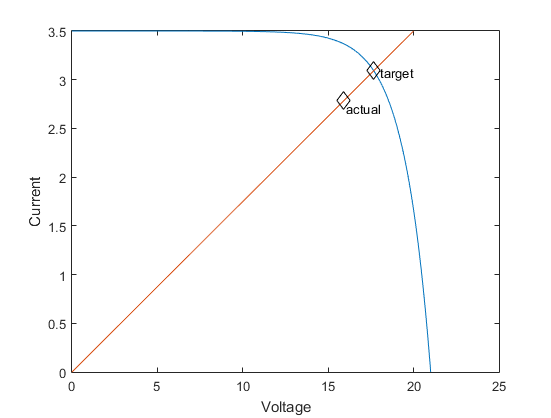
\includegraphics[width=.75\textwidth]{images/model/approx.png}
    \caption{Actual and target operating points}
    \label{fig:model:approx}
\end{figure}
The  intersection  is found  by  using  a  binary  search  algorithm,  which  is
converging slower than newton's method but more  stable  --- newton's method can
fail if $V_T$ in \eqref{eq:IV} is small.


\subsection{Using more than one curve}

If we want to use multiple curves to model the staircase characteristic shown in
figure \ref{fig:model:steps} we  need to determine which curve is applicable for
a given load. This process can be made less CPU intensive if we precalculate the
resistance-thresholds by finding the intersections between two curves.  There is
always exactly one intersection if  $V_{oc1} > V_{oc2}$ and $I_{sc1} < I_{sc2}$.
\todo{insert graph}

